One can normalize the quantities to unit-less quantities for the purpose of numerical calculation and rough ordering estimate. This chapter will establish some ordering estimate for certain cases.

\section{DIII-D pedestal}

The calculation is based on a DIII-D H mode shot175823. Figure\ref{fig:ne} and Figure\ref{fig:Te}. 

\begin{figure}[h] \centering
        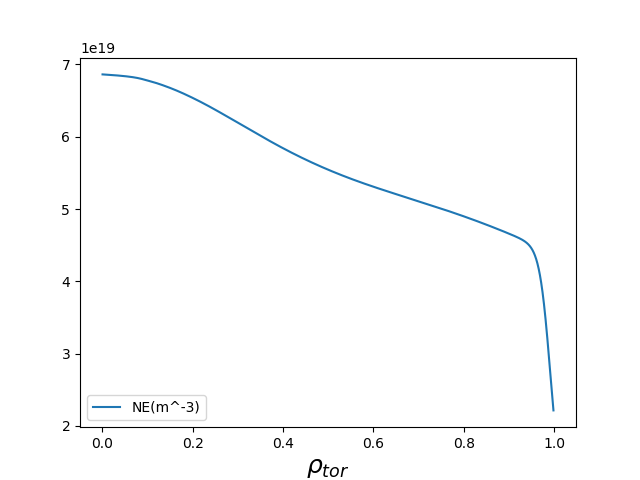
\includegraphics[width=1\textwidth]{Image/ne.png}
        \caption{The electron density}
        \label{fig:ne}
\end{figure}

\begin{figure}[h] \centering
        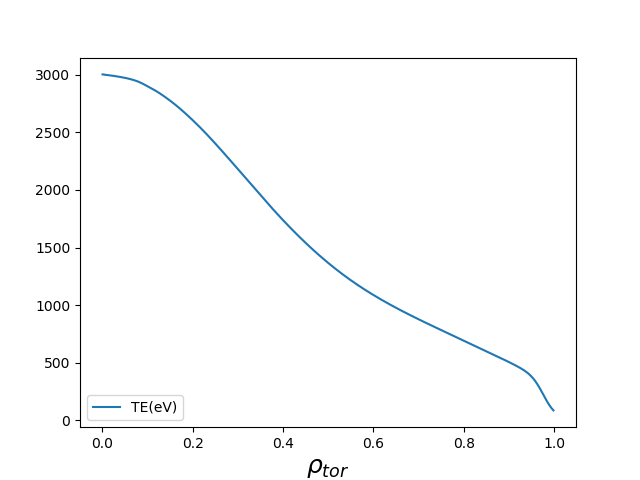
\includegraphics[width=1\textwidth]{Image/Te.png}
        \caption{The electron temperature}
        \label{fig:Te}
\end{figure}

At the mid pedastal(x/a=0.98) we have:\\
$a=0.67m$\\
$R=1.67m$\\
$B_0=2.2T$\\
$T_e=200eV$\\
$n_e=3.5\times 10^{19} /m^3$\\
$T_i=500eV$\\
$n_i=3.3\times 10^{19} /m^3$\\

People normalized frequency and growth rate in the unit of $c_s/a$

$c_s/a=\sqrt{\frac{\gamma k_B T}{M}}/a=282.9kHz$


Here are the unit-less quantities from a mid-pedestal of the DIII-D

$x=\frac{r}{a}=0.98$\\
$1/L_{n,e}=|\frac{1}{T_e}\frac{dT_e}{d x}|=25$\\
$1/L_{T,e}=|\frac{1}{T_e}\frac{dT_e}{d x}|=25$\\
$1/L_s=\frac{\hat{s}}{Rq}=\frac{1}{q}\frac{dq}{dx}=1$\\

\subsection{Typical waves}

$v_{th,s}=\sqrt{\frac{3 k_B T_s}{m_s}}$

Then $v_{th,i}=1.7\times 10^{5} m/s$

Diamagnetic Drift waves $\omega_{*e}=\frac{k_yT_e }{a L_n eB_0}=k_y*3.9*10^{23}$

Alfven wave $v_A=\frac{B_0}{\sqrt{4\pi m_in_i}}=1869m/s$

Cylotron frequency $\omega_c=\frac{e B_0}{m_i}=1.05\times 10^{8} rad/s$

Plamsa wave $\omega_p=\sqrt{\frac{n_0 e^2}{\epsilon_0 M}}=5.5\times 10^9 rad/s$

Gryoradius $\rho_i\approx \frac{v_{th,i}}{\omega_{c,i}}=1.6mm$




